
\documentclass{scrartcl}
\usepackage[dvipsnames,usenames, table]{xcolor} 

\usepackage[utf8]{inputenc}
\usepackage[T1]{fontenc}
\usepackage[english]{babel}
\usepackage[a4paper, margin=1in]{geometry}
\usepackage{lipsum}
\usepackage{amssymb}
\usepackage{libertine}
\usepackage{amsmath}
\usepackage{libertinust1math}
\usepackage[footnotes,definitionLists,hashEnumerators,smartEllipses,hybrid]{markdown}
\usepackage{amsthm}
\usepackage{framed}
\usepackage{mathtools}
\DeclarePairedDelimiter{\ceil}{\lceil}{\rceil}
\DeclarePairedDelimiter\floor{\lfloor}{\rfloor}

\usepackage{fancyhdr}
\usepackage{tikz}
\newcommand*\circled[1]{\tikz[baseline=(char.base)]{
            \node[shape=circle,draw,inner sep=2pt] (char) {#1};}}

\usepackage{graphicx}
\usepackage{microtype}
\usepackage[hidelinks]{hyperref}
\usepackage{tocloft}
\usepackage{lettrine}
\usepackage{GoudyIn}
\renewcommand{\LettrineFontHook}{\GoudyInfamily{}}
\newcommand{\DECORAR}[3][]{\lettrine[lines=3,loversize=.115,#1]{#2}{#3}}
\def\contentsname{\empty}

\newcommand{\tocr}{
\renewcommand\cftaftertoctitle{\par\noindent\hrulefill\par\vskip-0.65em}
\tableofcontents
\noindent\hrulefill
}


%BEGIN LISTINGDEF
\usepackage{listings}


\renewcommand{\ttdefault}{pcr}

\definecolor{listing-background}{rgb}{0.97,0.97,0.97}
\definecolor{listing-rule}{HTML}{B3B2B3}
\definecolor{listing-numbers}{HTML}{B3B2B3}
\definecolor{listing-text-color}{HTML}{000000}
\definecolor{listing-keyword}{HTML}{435489}
\definecolor{listing-identifier}{HTML}{435489}
\definecolor{listing-string}{HTML}{00999a}
\definecolor{listing-comment}{HTML}{8e8e8e}
\definecolor{listing-javadoc-comment}{HTML}{006CA9}

\lstdefinestyle{eisvogellistingstyle}{
	language=java,
	numbers=left,
	backgroundcolor=\color{listing-background},
	basicstyle=\color{listing-text-color}\small\ttfamily{}, % print whole listing small
	xleftmargin=0.8em, % 2.8 with line numbers
	breaklines=true,
	frame=single,
	framesep=0.6mm,
	rulecolor=\color{listing-rule},
	frameround=ffff,
	framexleftmargin=0.4em, % 2.4 with line numbers | 0.4 without them
	tabsize=4, %width of tabs
	numberstyle=\color{listing-numbers},
	aboveskip=1.0em,
	keywordstyle=\color{listing-keyword}\bfseries, % underlined bold black keywords
	classoffset=0,
	sensitive=true,
	identifierstyle=\color{listing-identifier}, % nothing happens
	commentstyle=\color{listing-comment}, % white comments
	morecomment=[s][\color{listing-javadoc-comment}]{/**}{*/},
	stringstyle=\color{listing-string}, % typewriter type for strings
	showstringspaces=false, % no special string spaces
	escapeinside={/*@}{@*/}, % for comments
	literate=
	{á}{{\'a}}1 {é}{{\'e}}1 {í}{{\'i}}1 {ó}{{\'o}}1 {ú}{{\'u}}1
	{Á}{{\'A}}1 {É}{{\'E}}1 {Í}{{\'I}}1 {Ó}{{\'O}}1 {Ú}{{\'U}}1
	{à}{{\`a}}1 {è}{{\'e}}1 {ì}{{\`i}}1 {ò}{{\`o}}1 {ù}{{\`u}}1
	{À}{{\`A}}1 {È}{{\'E}}1 {Ì}{{\`I}}1 {Ò}{{\`O}}1 {Ù}{{\`U}}1
	{ä}{{\"a}}1 {ë}{{\"e}}1 {ï}{{\"i}}1 {ö}{{\"o}}1 {ü}{{\"u}}1
	{Ä}{{\"A}}1 {Ë}{{\"E}}1 {Ï}{{\"I}}1 {Ö}{{\"O}}1 {Ü}{{\"U}}1
	{â}{{\^a}}1 {ê}{{\^e}}1 {î}{{\^i}}1 {ô}{{\^o}}1 {û}{{\^u}}1
	{Â}{{\^A}}1 {Ê}{{\^E}}1 {Î}{{\^I}}1 {Ô}{{\^O}}1 {Û}{{\^U}}1
	{œ}{{\oe}}1 {Œ}{{\OE}}1 {æ}{{\ae}}1 {Æ}{{\AE}}1 {ß}{{\ss}}1
	{ç}{{\c c}}1 {Ç}{{\c C}}1 {ø}{{\o}}1 {å}{{\r a}}1 {Å}{{\r A}}1
	{€}{{\EUR}}1 {£}{{\pounds}}1 {«}{{\guillemotleft}}1
	{»}{{\guillemotright}}1 {ñ}{{\~n}}1 {Ñ}{{\~N}}1 {¿}{{?`}}1
}
\lstset{style=eisvogellistingstyle}
\usepackage{tikz}

\usepackage{tikz-qtree}  
%END LISTINGDEF

\newcommand{\titleVar}{Exceptions in Java}
\newcommand{\authorVar}{David Zollikofer}
\newcommand{\es}{\varnothing}
\renewcommand{\tilde}{\sim}
\title{\titleVar}
%\date{\today}
%\author{\authorVar}


%making nice headers & footers
\pagestyle{fancy}
\fancyhf{}
\rhead{\titleVar}
\lhead{\authorVar}
\rfoot{Page \thepage}

\newtheorem{defn}{Definition}[section]


\begin{document}


\maketitle

\thispagestyle{fancy}

\section{Throwable in Java}

An exception is an event, which occurs during the execution of a program, that disrupts the normal flow of the program's instructions. The Java virtual machine immediately aborts code execution. Exceptions can be caused by:
\begin{itemize}
    \item serious runtime issues such as a stack overflow
    \item accessing attributes or calling methods of objects not pointing to a reference
    \item trying to write to a file with no permissions
    \item arithmetic exceptions - e.g. division by zero.
    \item programmer defined exceptions, e.g. non-conformable arguments
\end{itemize}

The process of stopping normal code execution is called  \textit{raising an exception or error}. It is important to note that all exceptions are objects. These objects must extend the \textsc{throwable} class  (which is a class and not an interface!). Java however already has two subclasses that are more convenient to extend. \textsc{Exception} and \textsc{Error}.


\begin{figure}[!h]
  \centering
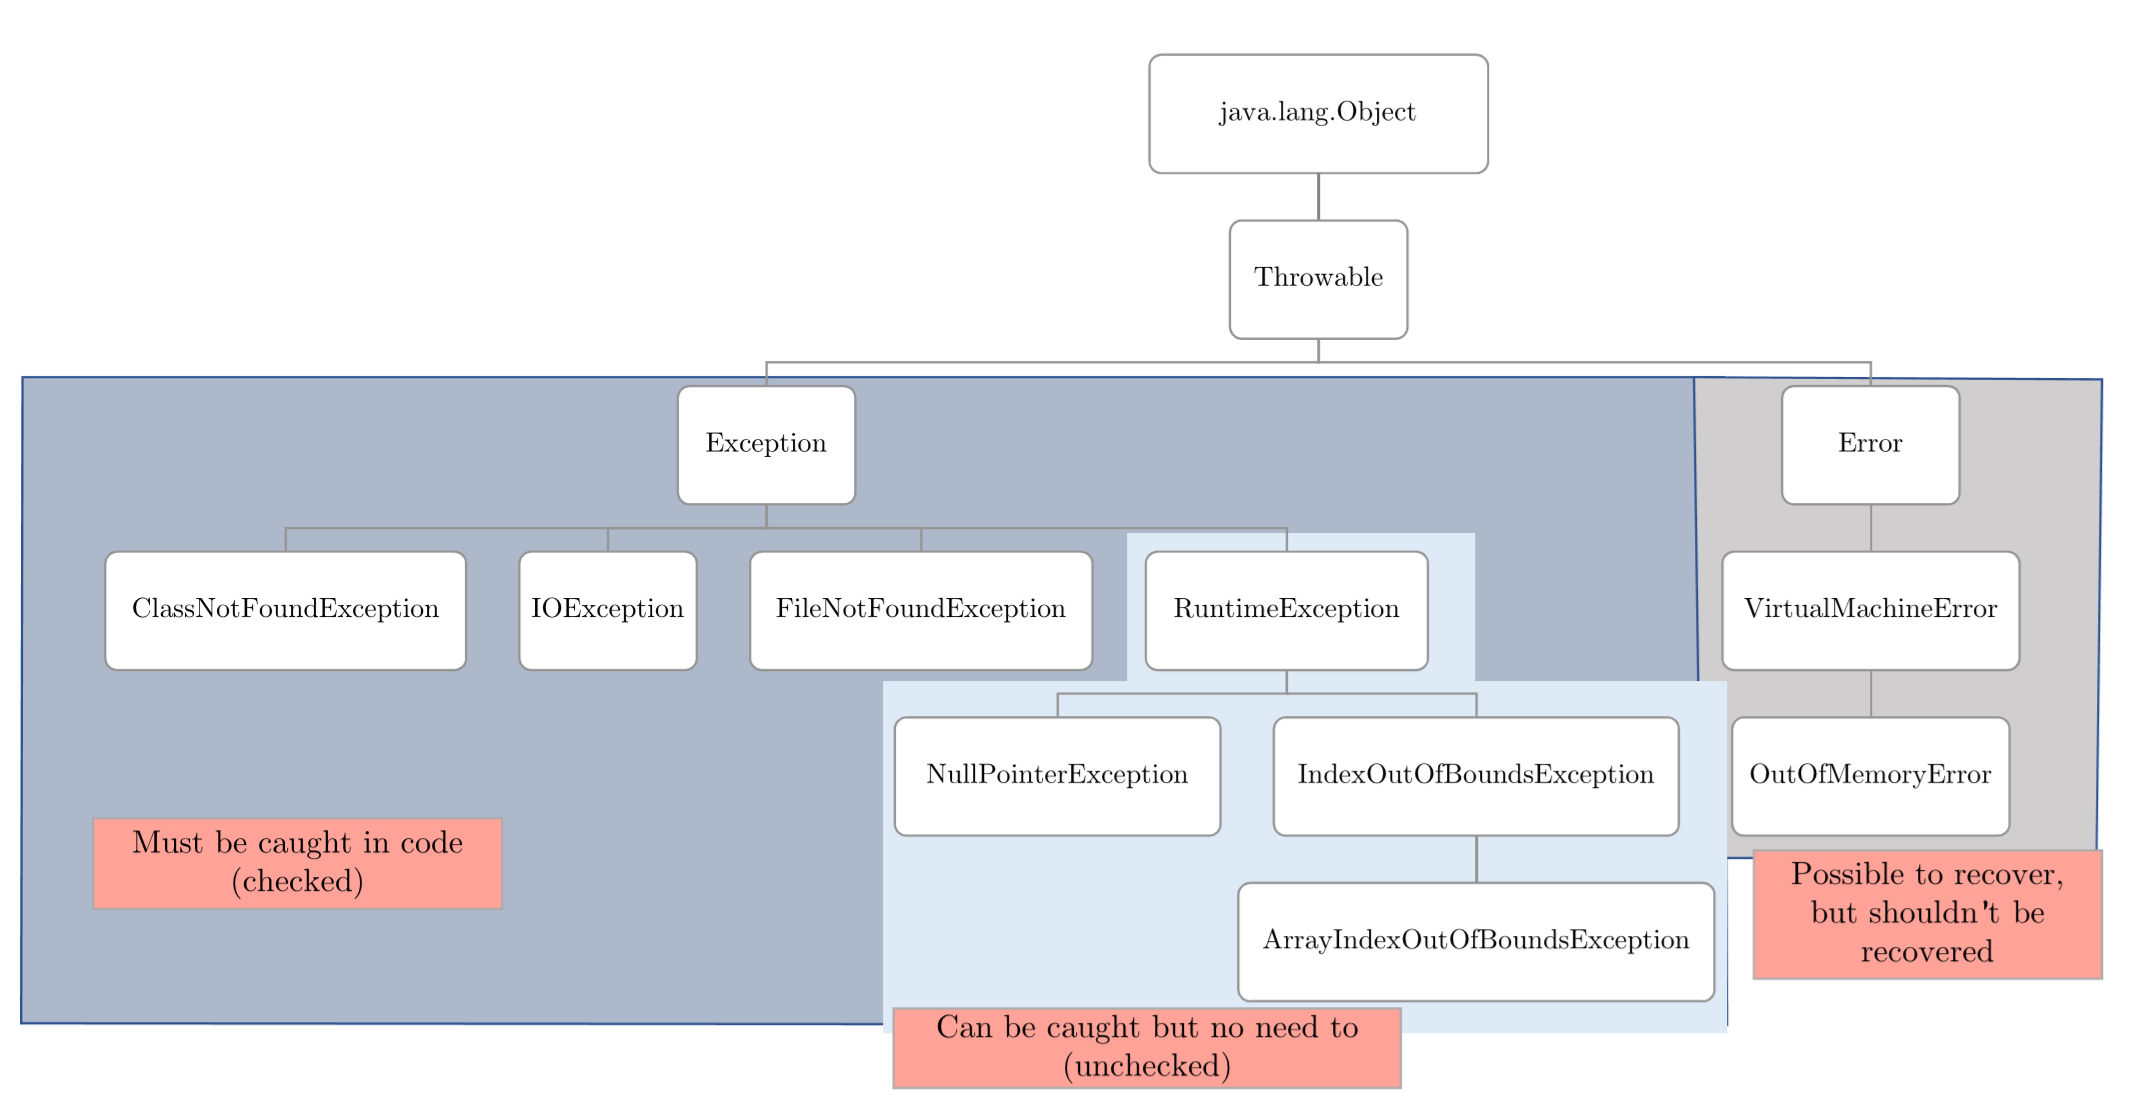
\includegraphics[width=\textwidth]{jerrs.png}
  \caption{non complete diagram of common Java Error/Exception objects}
\end{figure}
\begin{itemize}
    \item[Error] Indicates serious problems that a reasonable application should not try to catch. Most such errors are abnormal conditions. But can theoretically be caught.
    \item[Exception] The class Exception and its subclasses are a form of Throwable that indicates conditions that a reasonable application might want to catch.
 The class Exception and any subclasses that are not also subclasses of RuntimeException are checked exceptions.
    \item[RuntimeException] RuntimeException is the superclass of those exceptions that can be thrown during the normal operation of the Java Virtual Machine. RuntimeException and its subclasses are unchecked exceptions. Unchecked exceptions do not need to be declared in a method or constructor's throws clause if they can be thrown by the execution of the method or constructor and propagate outside the method or constructor boundary.
\end{itemize}

\section{Catching Exceptions}
The following shows the basic structure of error handling in Java.
\begin{lstlisting}[language=java]
try{
    // do some risky things
    russian_roulette();
} catch(Exception ex){
    ex.printStackTrace();
    // handle the error
}finally{
    cleanup();
    // will always run. resources such as streams can be closed in here.
}
\end{lstlisting}

You can also catch multiple errors simultaneously:
\begin{lstlisting}[language=java]
catch(NullPointerException ex){
    ex.printStackTrace();
}
catch(RuntimeException ex){
    ex.printStackTrace();
}
catch(Exception ex){
    ex.printStackTrace();
}
catch(Throwable ex){
    ex.printStackTrace();
}
\end{lstlisting}
it is important to note that if we first caught the \textsc{Throwable}, we could not have caught the \textsc{NullPointerException} later on since the latter is a subclass of the first. Alternatively in Java 7 one could also do the following:
\begin{lstlisting}[language=java]
catch(NullPointerException | RuntimeException | Exception ex){
    // useless example but shows how it works
    ex.printStackTrace();
}
\end{lstlisting}
In the catch block the type of the exception can be determined using the \textsc{typeof} keyword and case distinction.


\section{Throwing Exceptions / Errors}
To throw an exception in a program simply write:
\begin{lstlisting}[language=java]
throw new Exception();
\end{lstlisting}
If the error is a subclass of \textsc{RuntimeException} no further action is needed since the error being thrown is an unchecked error. However, if it doesn't extend \textsc{RuntimeException}, the \textsc{throw} must be surrounded by a \textsc{try catch} block, or the method signature must specify that an error will be thrown. 
\begin{lstlisting}[language=java]
void wontWork() throws Exception{
    throw new Exception();
}

void wontWork2(boolean b) throws NullPointerException, RuntimeException{
    if(b){
        throw new NullPointerException("oh no");
    } else {
        throw new RuntimeException("this is a message");
    }
}
\end{lstlisting}
You should note, that even though the second function will compile it is considered terrible style to throw more than one function.


\section{Defining Custom Exceptions}
This is actually very easy. One only needs to write a class extending a class that is already an exception or an error. This will give you all the behaviour of it's parent class. If you want a checked exception you usually extend \textsc{Exception}. For an unchecked one extends \textsc{RuntimeException}. Although one can extend \textsc{Throwable} or \textsc{Error} this is very bad style.

An example for an unchecked exception can be seen below:
\begin{lstlisting}[language=java]
class NotDuringOfficeHours extends RuntimeException
{
      // Parameterless Constructor
      public NotDuringOfficeHours() {}

      // Constructor that accepts a message
      public NotDuringOfficeHours(String message)
      {
         super(message);
      }
 }
\end{lstlisting}


\end{document}